\RequirePackage{luatex85,shellesc}
\documentclass[a4paper,9pt, addpoints, solutions]{exam}
\usepackage{pgf,tikz}
\usepackage{tikzsymbols}
\usepackage{pgfplots}
\usepackage{caption}
\usepackage{booktabs}
\usepackage{grffile}
\usepackage{amsmath}
% \linespread{1.1}
\usepackage{mathtools}
\usepackage{amssymb}
\usepackage{fontspec}
\setmainfont{opensans}
\usepackage[euler-digits]{eulervm}
\usepackage{pgfplots}
\usepackage{epsdice}
\usepackage{tfrupee}

% Title Page
\title{Information Theory 2019 \\ Tutorial 1} 
\date{\today}
\begin{document}
\maketitle

\section{Probability}
\begin{itemize}
    \item $\Omega$ : Set of all possible outcome.
    \item $Pr(x)$, probability of event $x$. $x$ must be in $\Omega$ ( $x \in \Omega$ ).
    \item  Sum of $Pr(x)$ for all $x$ in $\Omega$ must add to to 1 or $\sum_{x\in\Omega} Pr(x)= 1$
\end{itemize}

For example, when I roll a die it can land in six ways. For such a  die,
$\Omega$ consists of six outcomes (elements).  $\Omega={ \epsdice{1},
\epsdice{2}, \epsdice{3},\epsdice{4},\epsdice{5},\epsdice{6} }$. 

When die is fair, all outcomes are equally likely i.e. $Pr(\epsdice{1}) =
Pr(\epsdice{2}) = \ldots = Pr(\epsdice{6})$. Also $Pr(\epsdice{1}) +
Pr(\epsdice{2}) + \ldots + Pr(\epsdice{6}) = 1$. These two facts implies that
any outcome has the probability of $\frac{1}{6}$ or $Pr(x) = \frac{1}{6}$ for
any $x\in\Omega$.

\paragraph{Mean and variance}

Mean is often called expected value.

\begin{questions}

    \question Mean and variance
    \begin{parts}
        \part[2] Write the defination of mean and variance.
        \part[1] What is the expected value of a die. 
        \part[1] What is the expected value of a pair of dice.
    \end{parts}

\question[10]
Two lotteries sells 100 tickets every week. At the end of the week, one of these
tickets is selected randomly (each ticket is equally likely to win) and winner
is given 1 lakh rupees. Other 99 tickes gets nothing. You have enough money to
buy two tickets: you can buy both tickets from the same lottery or 1 from each
lotteries. Which strategy is \textit{better} given that you can play lottery enough
time.

\begin{solution} 
    If we buy two tickets from the same lottery (strategy \textbf{S1}), we have
    2% chance of winning \rupee 1 lakh, and 98% change of winning nothing.  If
    we buy both tickets from different lotteries (strategy \textbf{S2}), we have
    some change of winning \rupee 2 lakhs. Lets write down the probabilities.

    \begin{tabular}{c c c c}
        Strategy                    & \rupee 0     & \rupee 1 lakh & \rupee 2 lakh \\
        S1                          & 0.98         & 0.02          & \\
        S2                          & 0.9801       & 0.0198        & 0.0001 \\
    \end{tabular}

    With S2, we have slightly higher chance of not winning anything. But a non-zero
    chance of winning \rupee 2 lakhs. The expected value of win (mean) is same is
    both cases: $0 \times 0.98 + 0.02 \times 1 = 0.02$, and $0\times 0.9801 + 0.0198
    * 1 + 0.0001 * 2 = 0.02$. Yet the strategy looks different. After all if I buy
    100 tickets from same lottery, I am sure to win \rupee 1 lakh, but not with S2.

    Strictly speaker, which strategy is better is beyound the scope of this
    tutorial. All we can show how to do the calculations.  The standard deviation of
    S1 is ($\sqrt{0.98(0-0.02)^2+0.02(1-0.02)^2}$) 0.1386 and of S2 is
    0.1392265. We can say that S2 is \rupee 0.0006265 lakh riskier.

    Let play this lottery on computer since we can not play in real life.
    Figure @fig:1 shows the simultion. More often than not, S2 gives slightly
    higher return.

        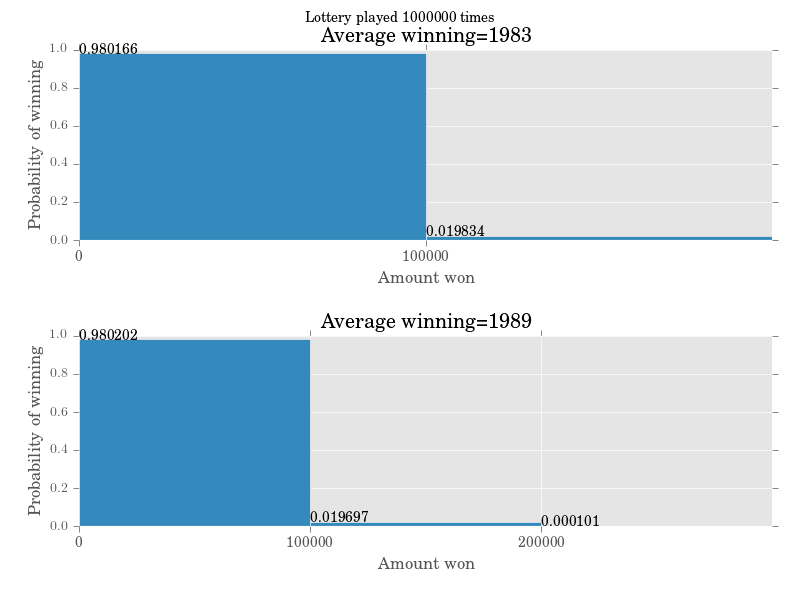
\includegraphics[width=1\textwidth]{./lotteries.py.png}
        \captionof{figure}{Second strategy is slightly better. On average, we might win more
            money with S2 given that we win \rupee 2 lakh. For very large number (almost
            infinite), both strategy will yield same results (since mean is same), however
            for large numbers of times lottery played, S2 seems to be more beneficial (as
        per simulations).}
        \label{fig:lottery}
\end{solution}

\question[10]

\textbf{(bonus)} In late 1990s, the Uttar Pradesh state government used to run
lottery. At the end of week if the number of ticket ended with the winning
digit, it would win 11 times the value of ticket. Each ticket has the
probability $\frac{1}{10}$ of winning the lottery.

In my village, local drunkard  came up with following algorithm which is sure
to make him rich.

Let fix the value of ticket to be \rupee 5 (winning amount \rupee 55).

\begin{itemize}
    \item On week 1, buy $n$ (assume 1) tickets with number ending with X.
    \item Repeat till you win: next week buy $2n$ ticket with number ending with X.
\end{itemize}

Inspired by his reasoning, if 100 people played the lottery using his algorithm
using their favourite X.  Assuming that everyone had 1 lakh rupee to start with,
how long it took (on average) for everyone to got bankrupt?

\begin{solution}
Let's solve a simpler problem first: what is the probability that
person gets bankrupt after n weeks. The number of tickets bought in n weeks are
$2^0 + 2^1 + \ldots + 2^n = \frac{2^{n+1}-1}{1}$. The cost of these tickets is
\rupee $5 \times (2^{n+1}-1)$. What is the expected value of winning during
these n weeks? The probability of winning during these $n$ weeks are $p2^0 +
p2^1 + \ldots p2^n$ where $p$ is the probability of any ticket winning i.e. 0.1.
So expected value of winning during these n weeks is \rupee$55p(2^{n+1} -
1)=\text{\rupee} 5.5 (2^{n+1}-1)$ which is higher than the cost of tickets. In
other words, we always (on average) end up making more money than spending.
\footnote{What's wrong which this argument?}

What if do not win any lottery for 15 weeks? There is a non-zero chance that
this might happen. If we don't win for 15 weeks, we spent all of our money and
go bankrupt. So the probability that we do not win anything for 15 weeks
definately one case where we go backrupt. 

Let assume that during $n$ weeks, we have won 1 lottery. There are n ways this
could happend: we won in first week, we won in second week, ..., we won in n'th
week. What is value of n before we go bankrupt in each of these cases? And what
are the probabilities of these events happening?

Lets assume that during $n$ weeks, we have $k$ times. How many ways we can win
these lotteries? Pick any k weeks from n weeks i.e. $^nC_k$. What is the value
of $n$ before we go bankrupt? What are the probabilities for these events
happening?

You see now, this is a complicated problem. There are many ways we can go
bankrupt and each way has non-zero probability? So how do we reach an answer? We
can simulate the process or we can come up with an smart solution to sum up all
the probable ways in which a person can go banckrupt. Therefore getting the
probability of a person going backrupt after n weeks.

%\begin{figure}
%    \includegraphics[]{./lottery_up.py.png}
%    \caption{In my approximately accurate simulation, it usually takes less than 20 weeks
%        for everyone to go backrupt. Columns in second suplot, shows the fortune of each
%    individuals. It fluctuates rapidly  after week 10.}
%\end{figure}
\end{solution}

\paragraph{Roll the dice\footnote{never say die}, play the cards, flip the coins}

\question For a pair of dice, write $\Omega$.
\begin{parts}
    \part[2] Consider $\epsdice{1}\epsdice{4}$ and $\epsdice{4}\epsdice{1}$ etc. as
distinct events.
    \part[3] Consider $\epsdice{1}\epsdice{5}$ and $\epsdice{5}\epsdice{1}$ etc. as same
event.
    \part[3] \textbf{(bonus)} Repeat the problem for 4 dice. You can use computer program to
check your results.
\end{parts}

\question[5] A loaded dice is given as $Pr(\epsdice{1})=\frac{1}{2}$,
$Pr(\epsdice{2})=\frac{1}{4}$, $Pr(\epsdice{3}) = Pr(\epsdice{4}) = Pr(
\epsdice{5}) = Pr(\epsdice{6}) = \frac{1}{16}$. Write down $\Omega$ and
probability of each event ($Pr(x),\; x \in \Omega$) when we roll two dice.
\begin{enumerate}
    \item Both are loaded.
    \item One is loaded, other is 'fair'.
\end{enumerate}
Assume that $\epsdice{3}\epsdice{4}$ and $\epsdice{4}\epsdice{3}$ etc. are the
same event.

\begin{solution}
Solution No given.
\end{solution}

\question[5]
Your TA flipped a Rs. 1 coin repeatedly. Once he got two head in succession,
he noted down the number of flips. He got the following sequence:
\verb|6,3,6,8,7,12,16,2,3,2| \footnote{He wanted to do 20 samples, but he flipped out after 10.}
Fortunately others have also done such excercise. I was able to get following
data from two universities.

\verb|3,2,3,5,10,2,6,6,9,2|     (Stanford, 1979)
\verb|10,2,10,7,5,2,10,6,10,2|  (Princeton, 1987)

\begin{parts}
    \part[2] Compute (umm. estimate) the mean and variance of these sequences.
    \part[3] bonus Based on these sequence, can you estimate the probability
    that coin used was not 'fair'? If yes, estimate. If no, why not?
\end{parts}

\begin{solution}
    

\begin{tabular}{c c  c}
 Coin         & mean & $\sqrt{\text{variance}}$ \\
NCBS 2017     & 6.5  & 4.34  \\
Stanford 1979 & 4.79 & 2.78  \\
Princeton 1987& 6.4  & 3.35  \\
\end{tabular}

The answer is no and its not easy to explain.
Lets call this process X. Lets take an extreme case: NCBS 2017 series was the
following: 2,2,2,2,2,2,2,2,2,2 i.e. all 20 flips gave us heads. Can we say this
was definately a loaded coin? What is the probability that this sequence came
out of a fair coin? Or what is the probability of getting 20 heads in
succession? Ans is $(\frac{1}{2})^{20}$. It is non-zero!

What is the mean and variance of X for a fair coin anyway?  \footnote{mean=6,std=4.7}
\end{solution} 

\paragraph{Typical dressing}

\question[5]
A man has a non-magical wardrobe containing 10 shirts, 10 pants, 20 pairs of
socks, 10 pairs of shoes, 30 hats, and 50 neck-ties.  He is allowed to pick 6
items everyday. Whenever he chooses 1 shirt, 1 pant, 1 pair of
shoes, 1 pair of socks, 1 hat and 1 neck-tie, we call is 'typical garments'.

\begin{parts}
    \part[2] How many ways he can choose 6 items? 
    \begin{solution}
        There are total 130 items.  For first item, we have 130 choices,
        for second item, we have 129 choices etc. Total choices are $130 \times 129
        \times 128 \ldots 125$.
    \end{solution}

    \part[3]How many ways he can dress himself 'typically'?
    \begin{solution}
        He has to pick 1 items of each type. How many ways he can choose 1
        shirt out of 10 shirts? 10. Similarly there are 30 ways to pick 30 hats etc.
        Total typical dressings are $10 \times 10 \times 20 \times 10 \times 30 \times
        50$.
    \end{solution}

    \part[3] In a slightly off-beat world, a typical garmets contains at least 1
    shirt, 1 pant, and 1 pair of shoes. Rest of the 6 garmets chould be
    anything. How many ways he can dress himself 'typically'?
    \begin{solution}
        Solution Let see he pick required 1 shirt first. There are 10 ways. Next he
        picks required 1 pant, there are 10 ways. Similarly there are 10 ways for
        picking required 1 pair of shoes. Left are 3 garmets and they could be anything.
        How many ways he can pick 3 items out of 9 shirts, 9 pants, 10 pairs of shoes,
        20 pairs of socks, 30 hats and 50 neck-ties (total 127). Go back to problem 1. Ans is 
        $127 \times 126 \times 125$ for this part. So total ways to dress oneself
        typically is $10 \times 10 \times 10 \times 127 \times 126 \times 125$.
    \end{solution}
\end{parts}

\section{Some calculus}

\question $log_2 x = n \iff 2^n = x$
\begin{parts}
    \part[1] Show/prove/argue that $0 \log 0 = 0$.
    \part[2] Show that $\log_x y = \frac{\log_a y}{\log_a x}$.
    \part[2] Plot (show your work) $x \log(x) + (1-x) \log (1-x)$ where $0 \le x \le 1$.
\end{parts}

\begin{solution}
Solution Not given.
\end{solution}

\end{questions}

\end{document}          
